\documentclass{article}
\usepackage[]{graphicx}
\usepackage[]{xcolor}
\usepackage{alltt}
\usepackage[left=2.3cm,right=2.8cm, top = 2.2cm, bottom = 3cm]{geometry}
\usepackage{amsmath}
\usepackage{amssymb}
\usepackage{natbib}
\PassOptionsToPackage{hyphens}{url}
\usepackage{url} 
\usepackage[disable]{todonotes}
\usepackage{multicol}
\usepackage{rotating}
\usepackage{booktabs}
\usepackage[colorlinks=false]{hyperref} 
\setlength{\parskip}{\baselineskip}%
\setlength{\parindent}{0pt}%
\urlstyle{same}
\usepackage{lineno}
\linenumbers
\bibliographystyle{apalike}
%\bibliographystyle{vancouver}

% to handle authorship footnotes as numbers:
\makeatletter
\let\@fnsymbol\@arabic
\makeatother

\newcommand{\ra}[1]{\renewcommand{\arraystretch}{#1}}
\newcommand{\changed}[1]{#1}

% to write the simulated as iid symbol: 
\newcommand{\distas}[1]{\mathbin{\overset{#1}{\kern\z@\sim}}}%


\begin{document}

\appendix
\section{Supplementary information}

\renewcommand{\thefigure}{SI.\arabic{figure}}
\setcounter{figure}{0}
\renewcommand{\thetable}{SI.\arabic{table}} \setcounter{table}{0}

\subsection{Alternative Formulation of the WIS}
\label{sec:alternative-wis}

Instead of defining the WIS as an average of scores for individual quantiles, we can define it using an average of scores for symmetric predictive intervals. For a single prediction interval, the interval score (IS) is computed as the sum of three penalty components, dispersion (width of the prediction interval), underprediction and overprediction,  
%
\begin{linenomath*}
\begin{align}
 IS_\alpha(F,y) &= (u-l) + \frac{2}{\alpha} \cdot (l-y) \cdot \boldsymbol{1}(y \leq l) + \frac{2}{\alpha} \cdot (y-u) \cdot \boldsymbol{1}(y \geq u) \\
 &= \text{dispersion} + \text{underprediction} + \text{overprediction},    
\end{align}
\end{linenomath*}
%
where $\boldsymbol{1}()$ is the indicator function, $y$ is the observed value, and $l$ and $u$ are the $\frac{\alpha}{2}$ and $1 - \frac{\alpha}{2}$ quantiles of the predictive distribution, i.e. the lower and upper bound of a single central prediction interval. For a set of $K^*$ prediction intervals and the median $m$, the WIS is computed as a weighted sum, 
\begin{linenomath*}
\begin{equation}
\text{WIS} = \frac{1}{K^* + 0.5} \cdot \left(w_0 \cdot |y - m| + \sum_{k = 1}^{K^*} w_k \cdot IS_{\alpha_{k}}(F, y)\right),    
\end{equation} 
\end{linenomath*}
where $w_k$ is a weight for every interval. Usually, $w_k = \frac{\alpha_k}{2}$ and $w_0 = 0.5$. 

\begin{figure}[h!]
    \centering
    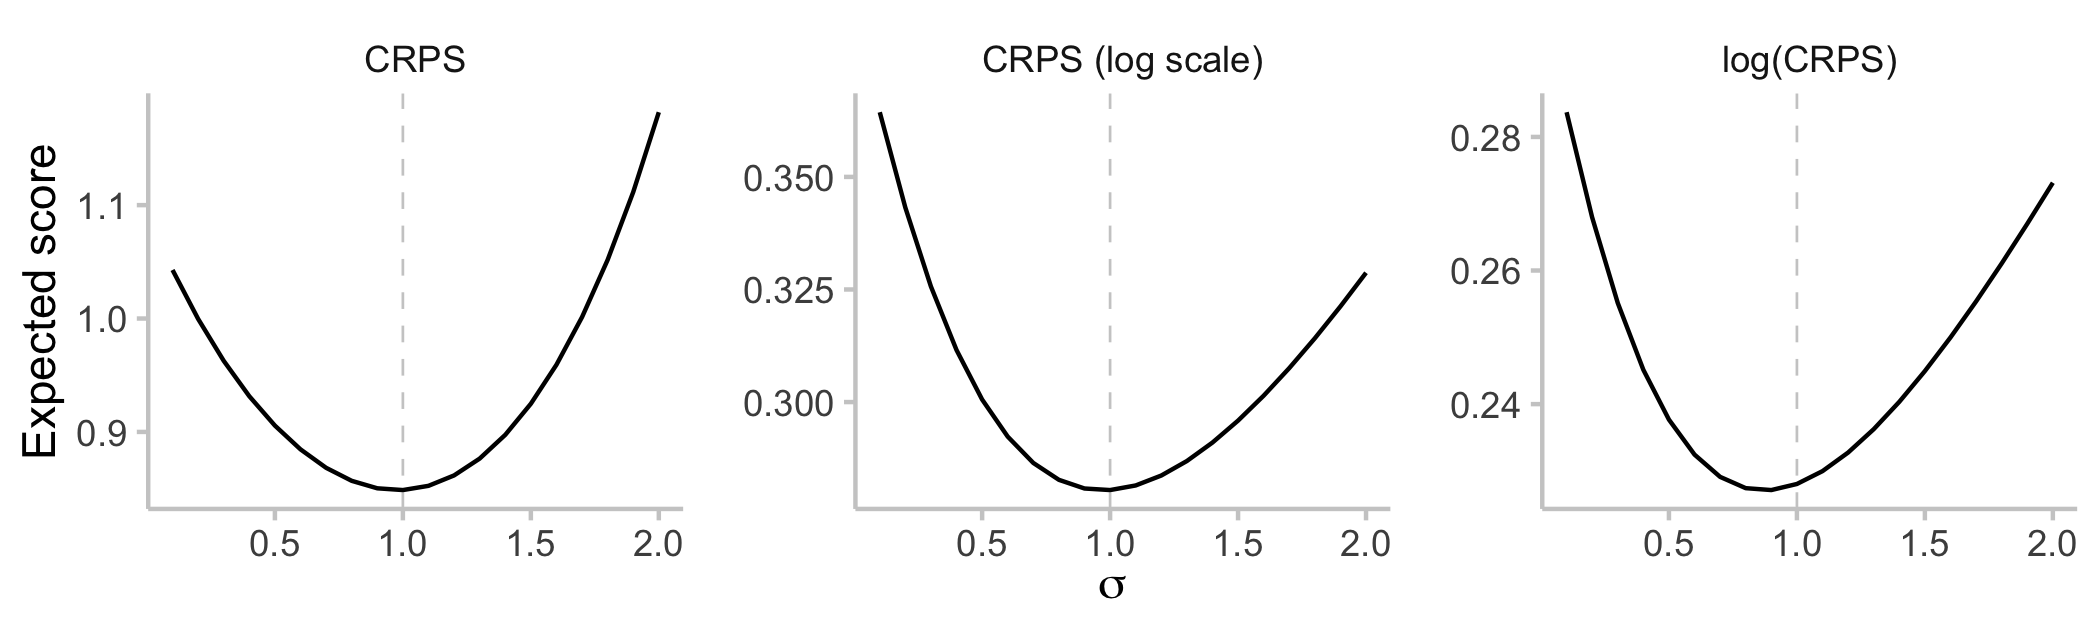
\includegraphics[width=0.99\textwidth]{../output/figures/example-log-first.png}
    \caption{Illustration of the effect of applying a transformation after scoring. We assume $Y \sim \text{LogNormal}(0, 1)$ and evaluate the expected CRPS for predictive distributions $\text{LogNormal}(0, \sigma)$ with varying values of $\sigma \in [0.1, 2]$. For the regular CRPS (left) and CRPS applied to log-transformed outcomes (middle), the lowest expectation is achieved for the true value $\sigma = 1$. For the log-transformed CRPS, the optimal value is  0.9, i.e. there is an incentive to report a forecast that is too sharp. The score is therefore no longer proper.}
    \label{fig:log-improper}
\end{figure}



\begin{figure}[h!]
    \centering
    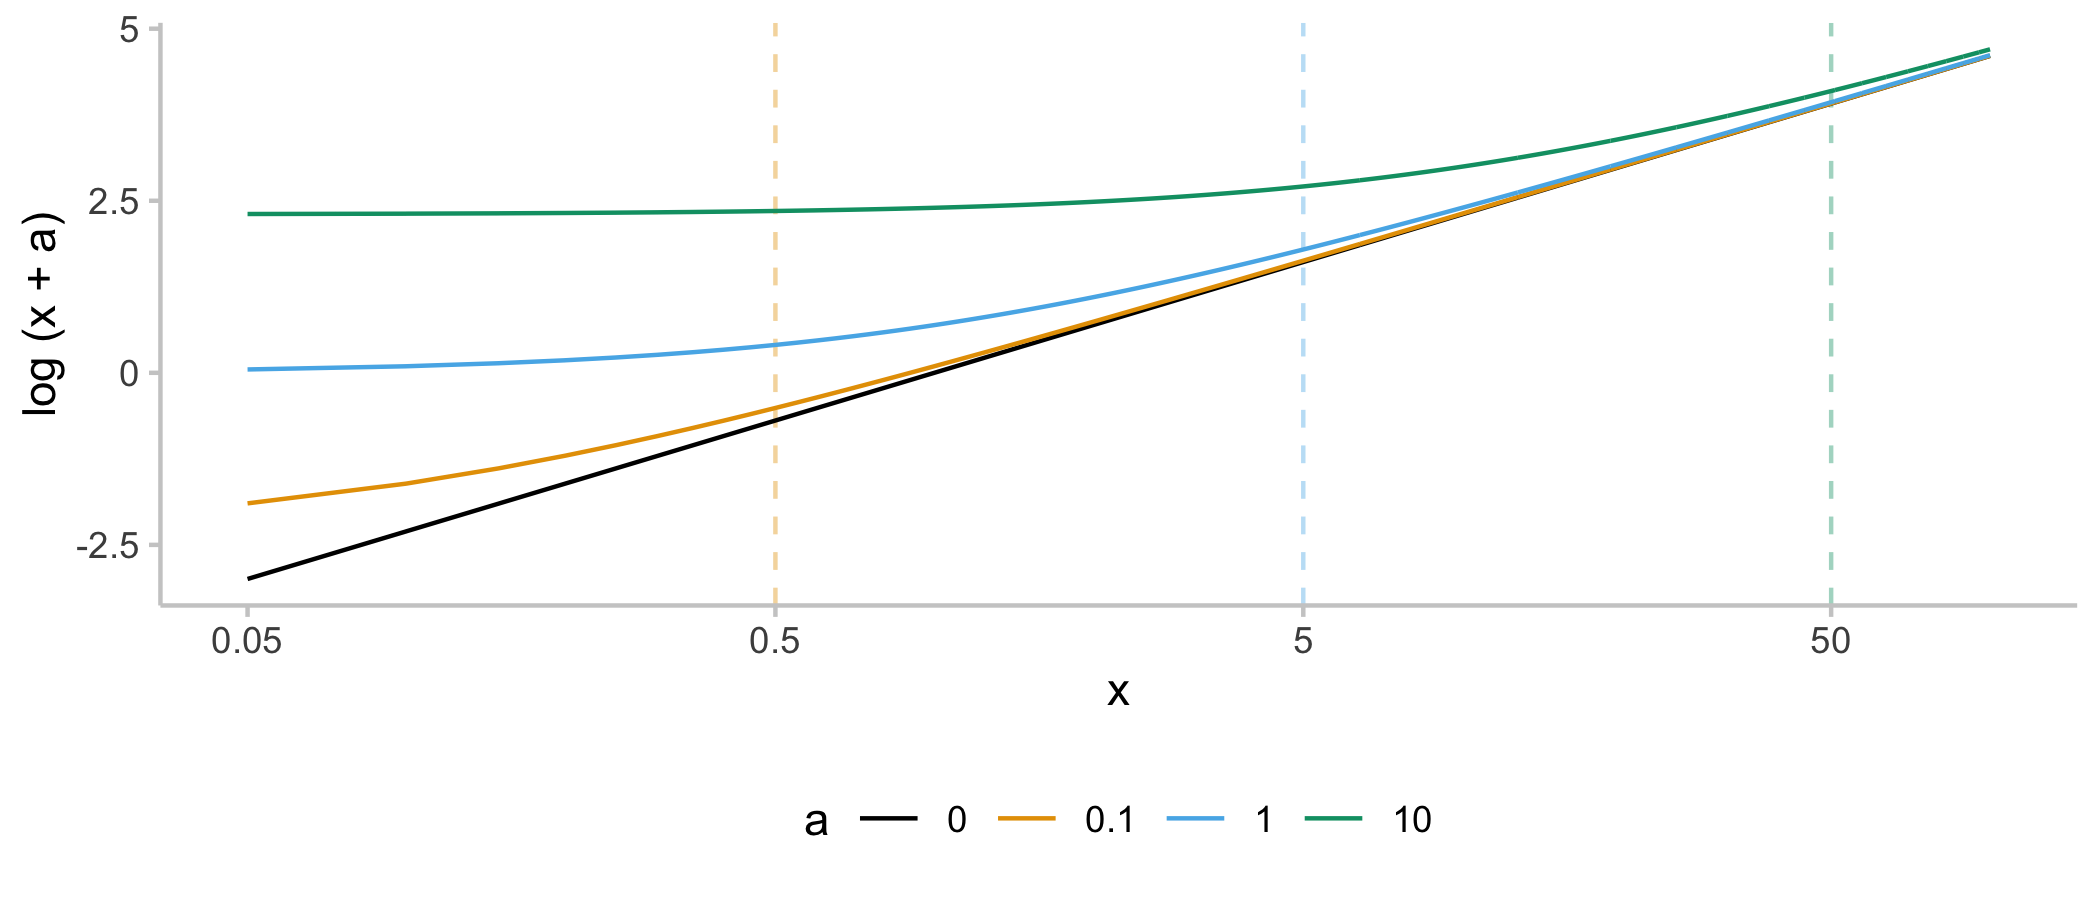
\includegraphics[width=0.99\textwidth]{../output/figures/illustration-effect-offset-log.png}
    \caption{Illustration of the effect of adding a small quantity to a value before taking the natural logarithm. For increasing x, all lines eventually approach the black line (representing a transformation with no offset applied).
    For a given solid line, the dashed line of the same colour marks the x-value that  is equal to 5 times the corresponding offset. It can be seen that for $a$ values smaller than one fifth of the transformed quantity, the effect of adding an offset is generally small. When choosing a suitable $a$, the trade-off is between staying close to the interpretation of a pure log-transformation (choosing a small $a$) and not giving excessive weights to small observations (by choosing a larger $a$, see Figure 6).}
    \label{fig:illustration-effect-log-offset}
\end{figure}


\begin{figure}[h!]
\centering
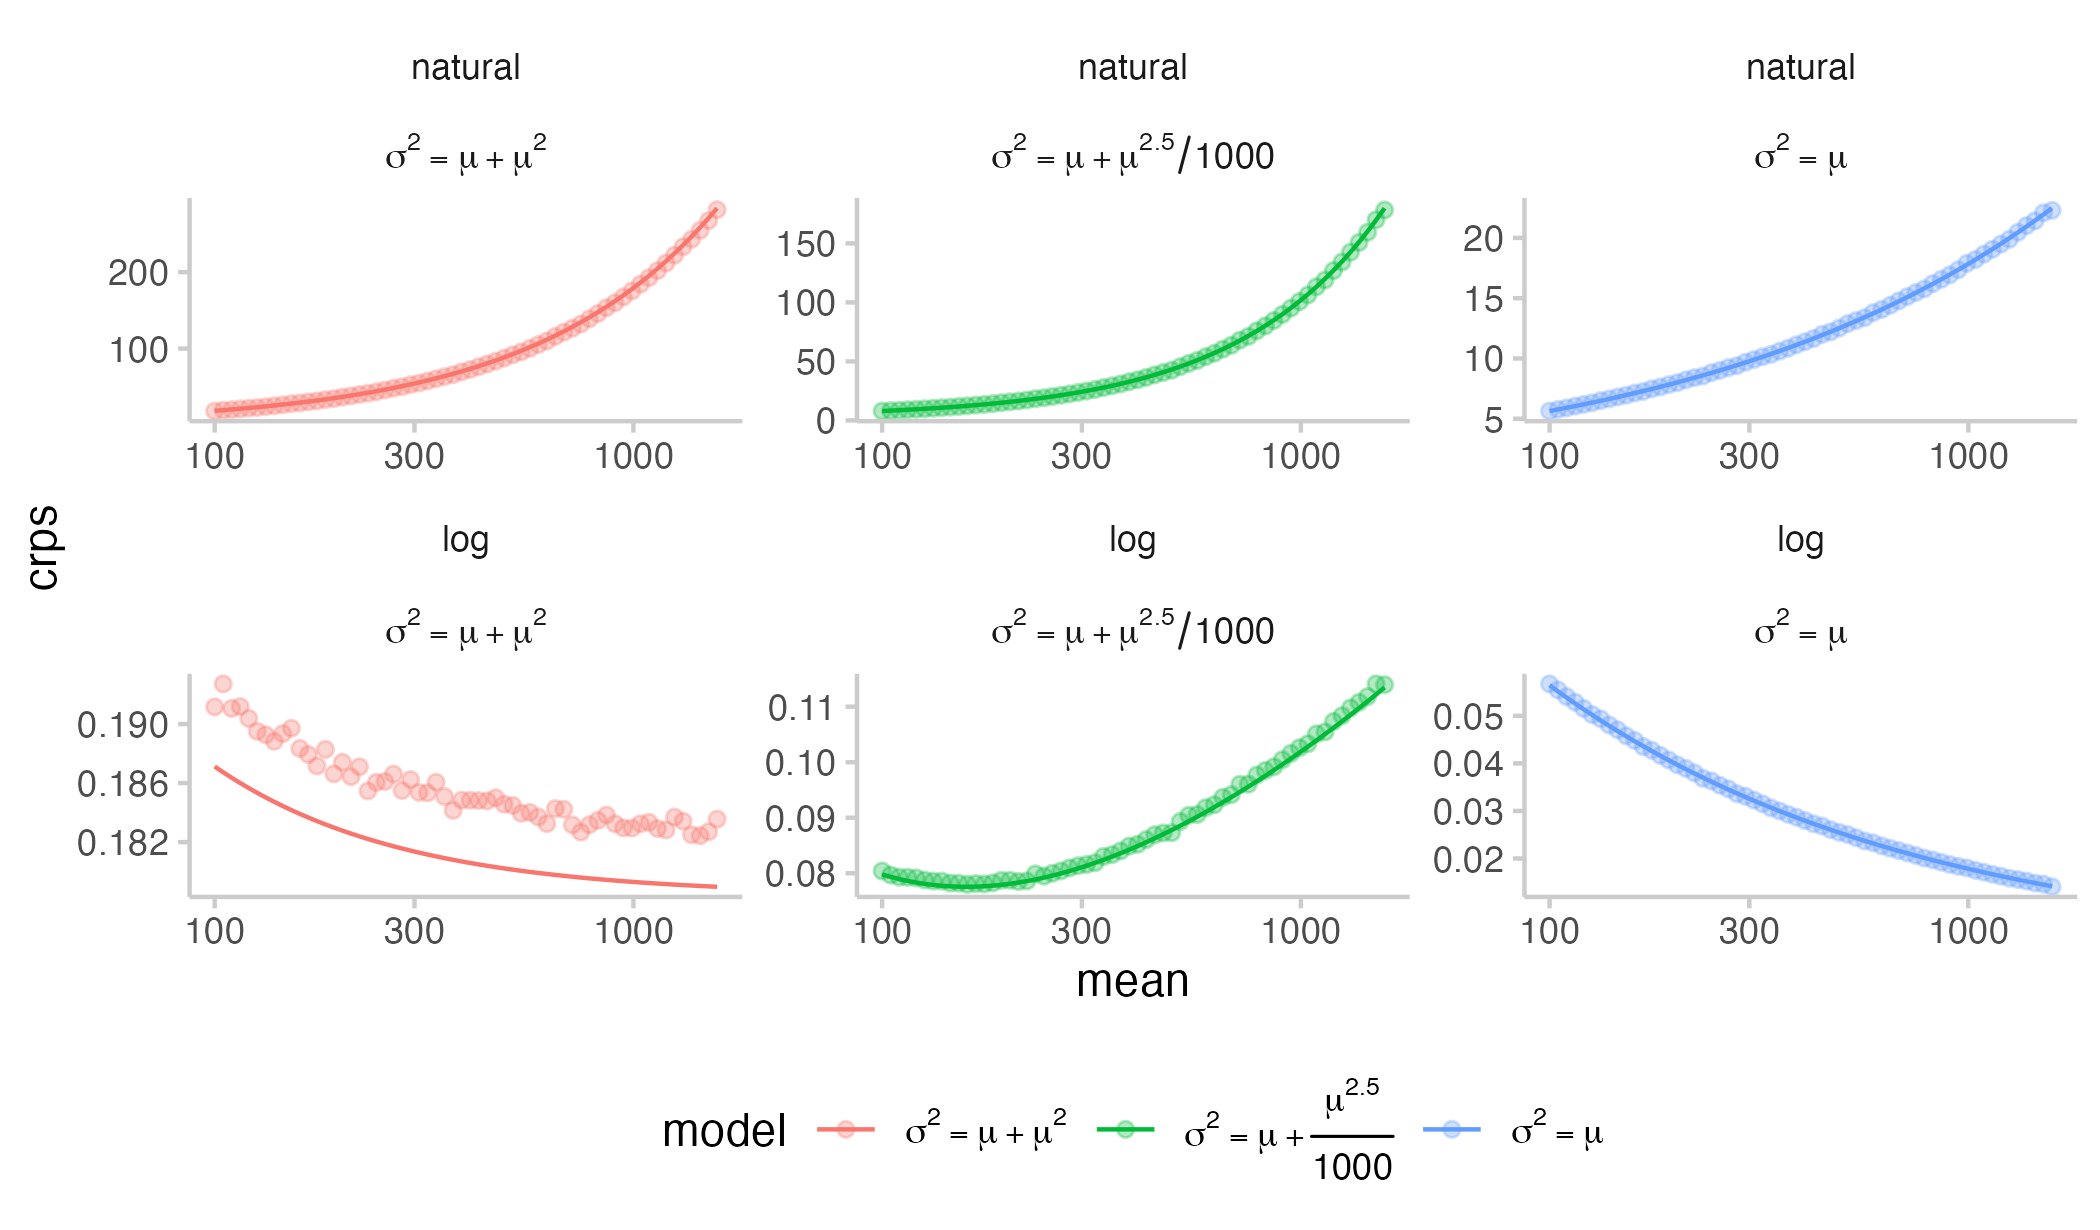
\includegraphics[width = 1\textwidth]{../output/figures/SIM-score-approximation.png}
\caption{
This is using the approximation detailed in the theoretical discussion on model rankings (see also Fig 2). Expected CRPS scores are shown for three different distributions once on the natural scale (top row) and once scored on the log scale (bottom row).
}
\label{fig:score-approx}
\end{figure}










%%%%%%%%%%%%%%%%%%%%%%%%%%%%%%%%%%%%%%%%
% HUB plots %




\begin{table}[h!]
    \centering
\begin{tabular}{lllcc}
\toprule
target type & quantity & measure & natural & log\\
\midrule
Cases & Observations & mean & 61979 & 9.19\\
Cases & Observations & sd & 171916 & 2.10\\
Cases & Observations & var & 29555122130 & 4.42\\
Deaths & Observations & mean & 220 & 3.89\\
Deaths & Observations & sd & 435 & 1.96\\
\addlinespace
Deaths & Observations & var & 189051 & 3.83\\
Cases & WIS & mean & 15840 & 0.27\\
Cases & WIS & sd & 53117 & 0.28\\
Deaths & WIS & mean & 31 & 0.23\\
Deaths & WIS & sd & 65 & 0.28\\
\bottomrule
\end{tabular}
    \caption{Summary statistics for observations and scores for forecasts from the ECDC data set.}
    \label{tab:HUB-summary}
\end{table}

\begin{figure}[h!]
    \centering
    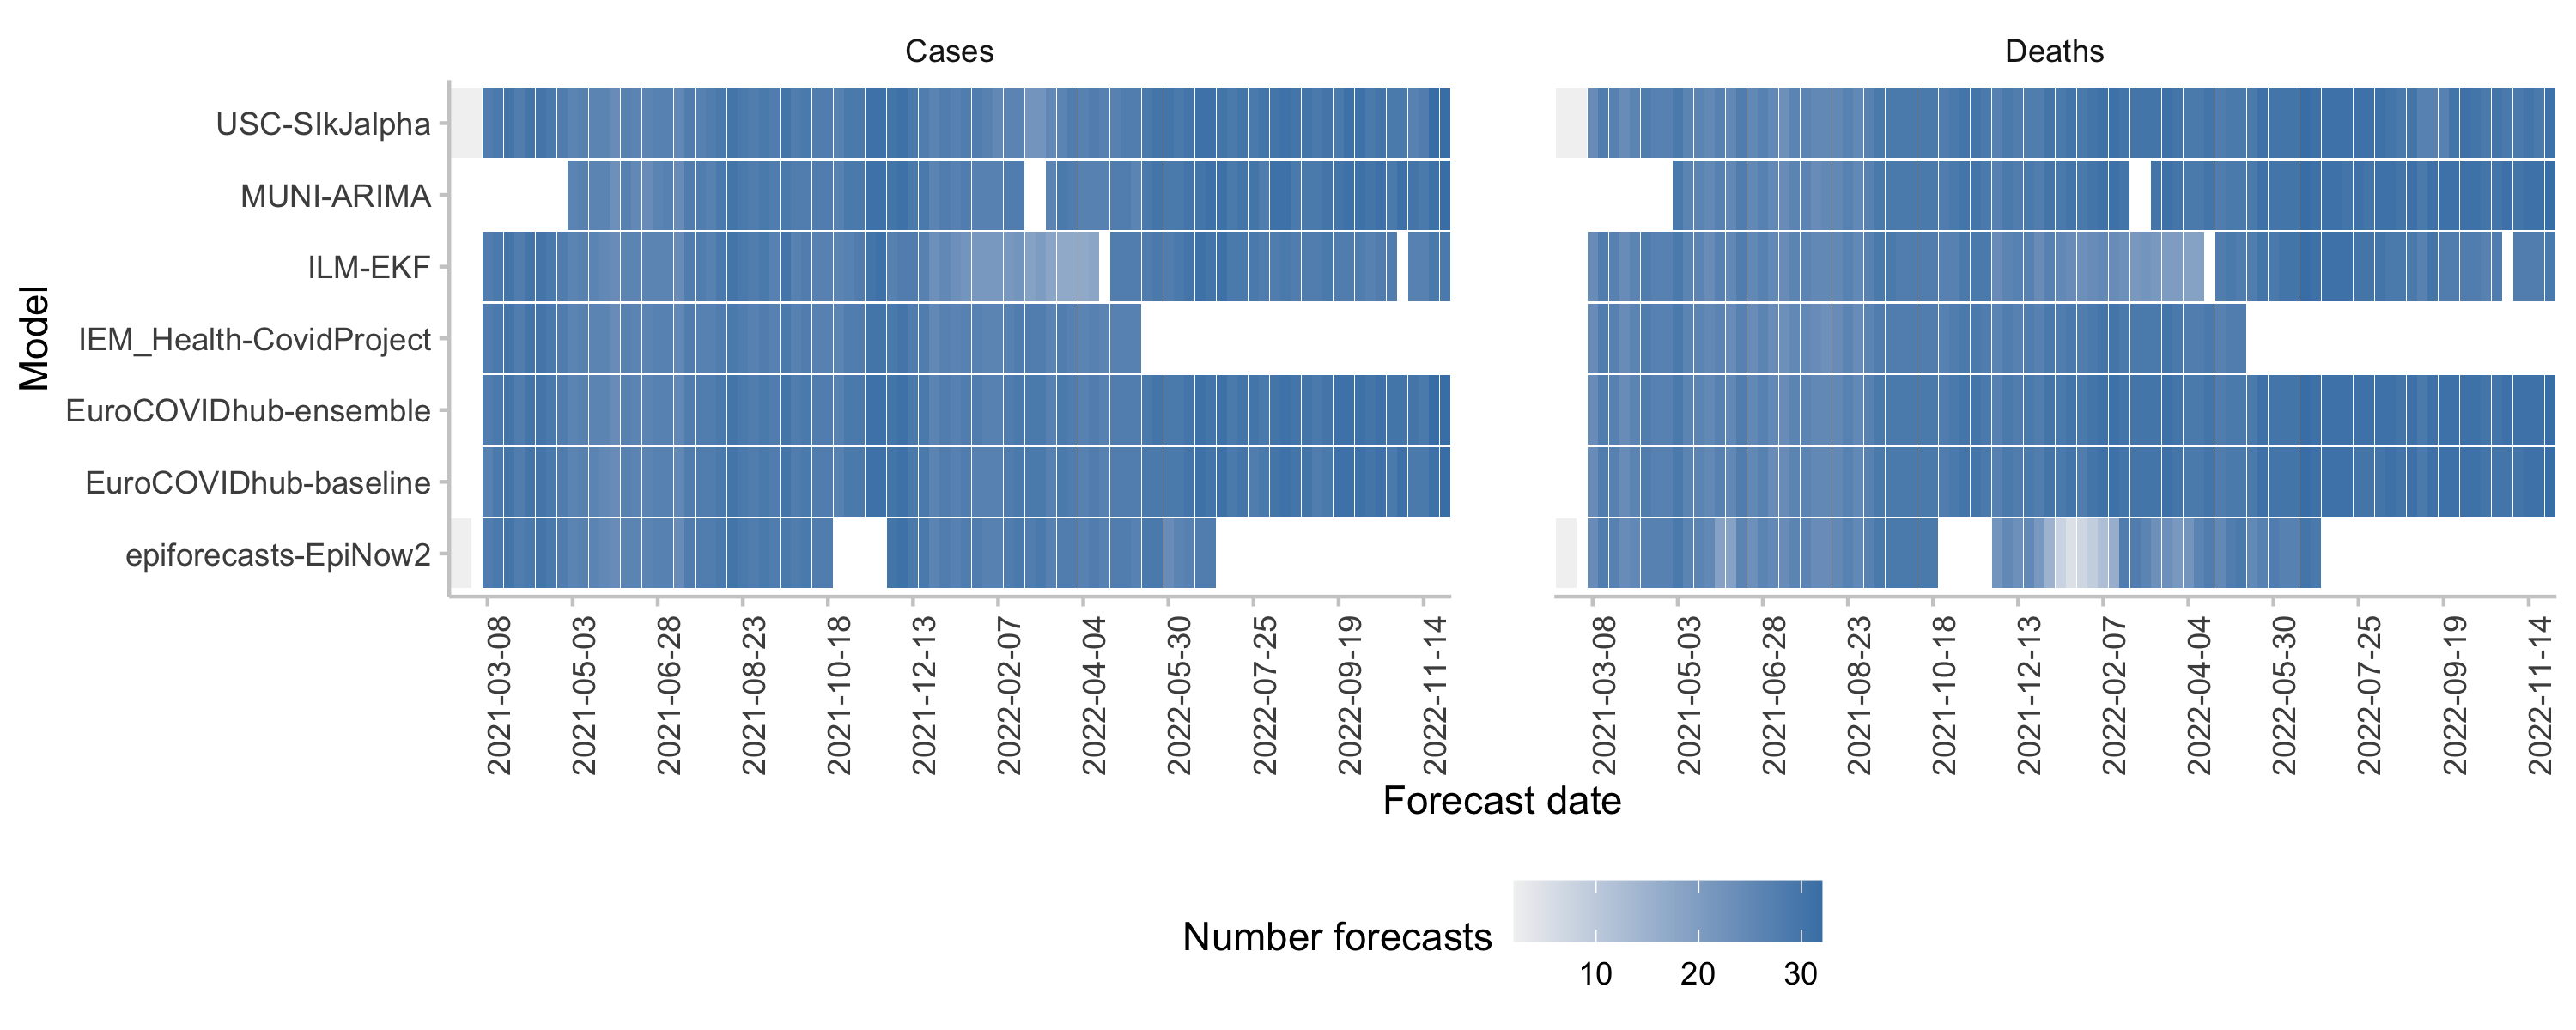
\includegraphics[width=0.99\textwidth]{../output/figures/number-avail-forecasts.png}
    \caption{
    Number of forecasts available from different models for each forecast date. 
    }
    \label{fig:HUB-num-avail-models}
\end{figure}


\begin{figure}[h!]
    \centering
    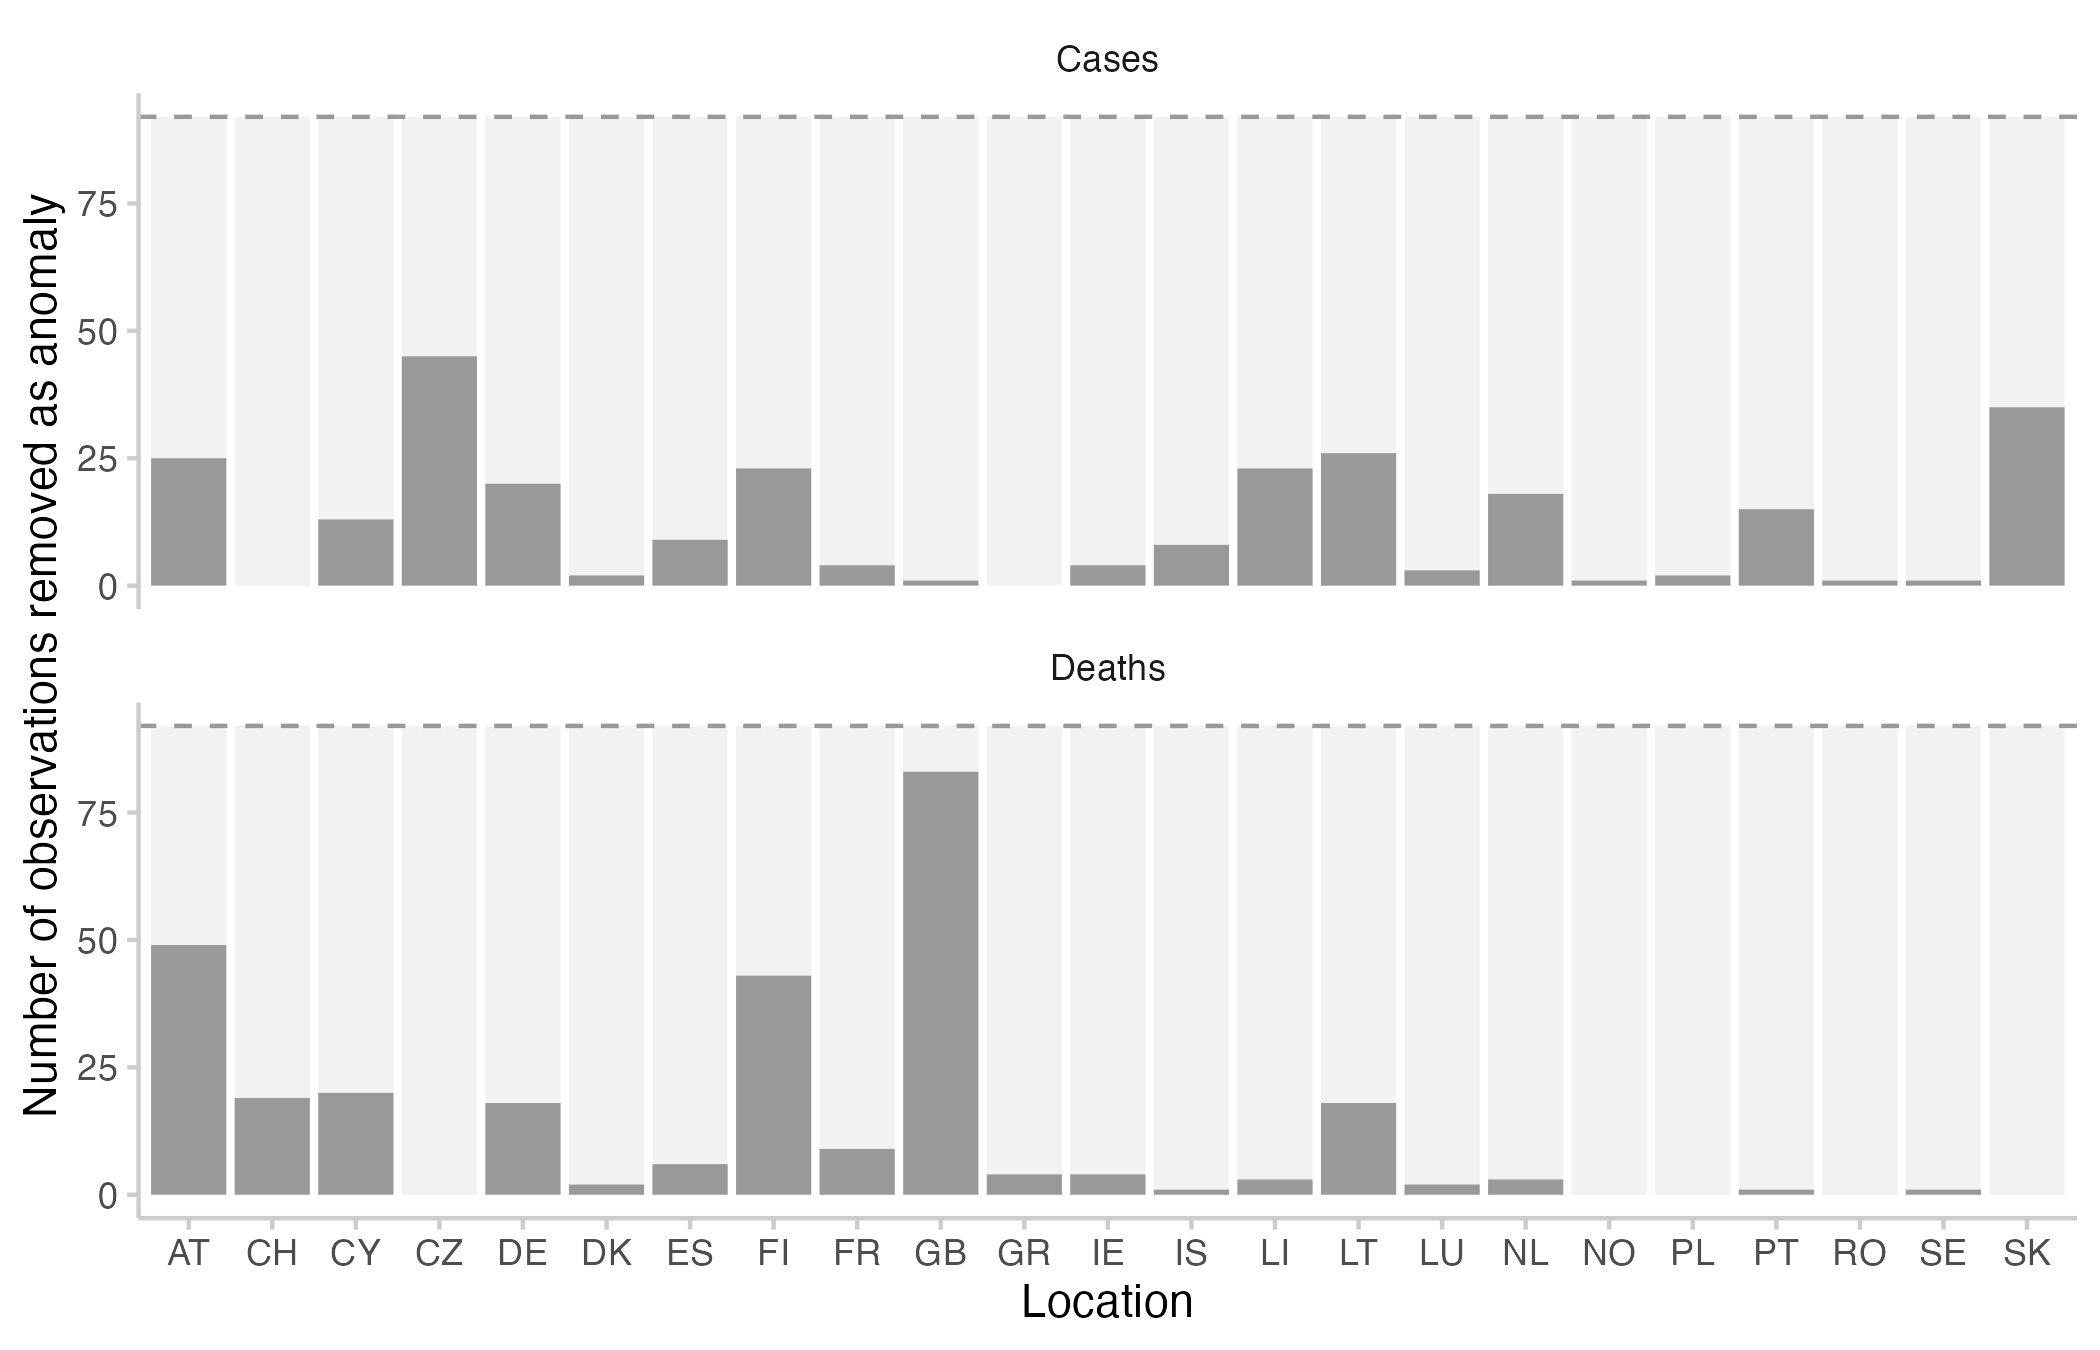
\includegraphics[width=0.99\textwidth]{../output/figures/number-anomalies.png}
    \caption{
    Number of observed values that were removed as anomalous. The values were marked as anomalous by the European Forecast Hub team. 
    }
    \label{fig:number-anomalies}
\end{figure}

\begin{figure}[h!]
    \centering
    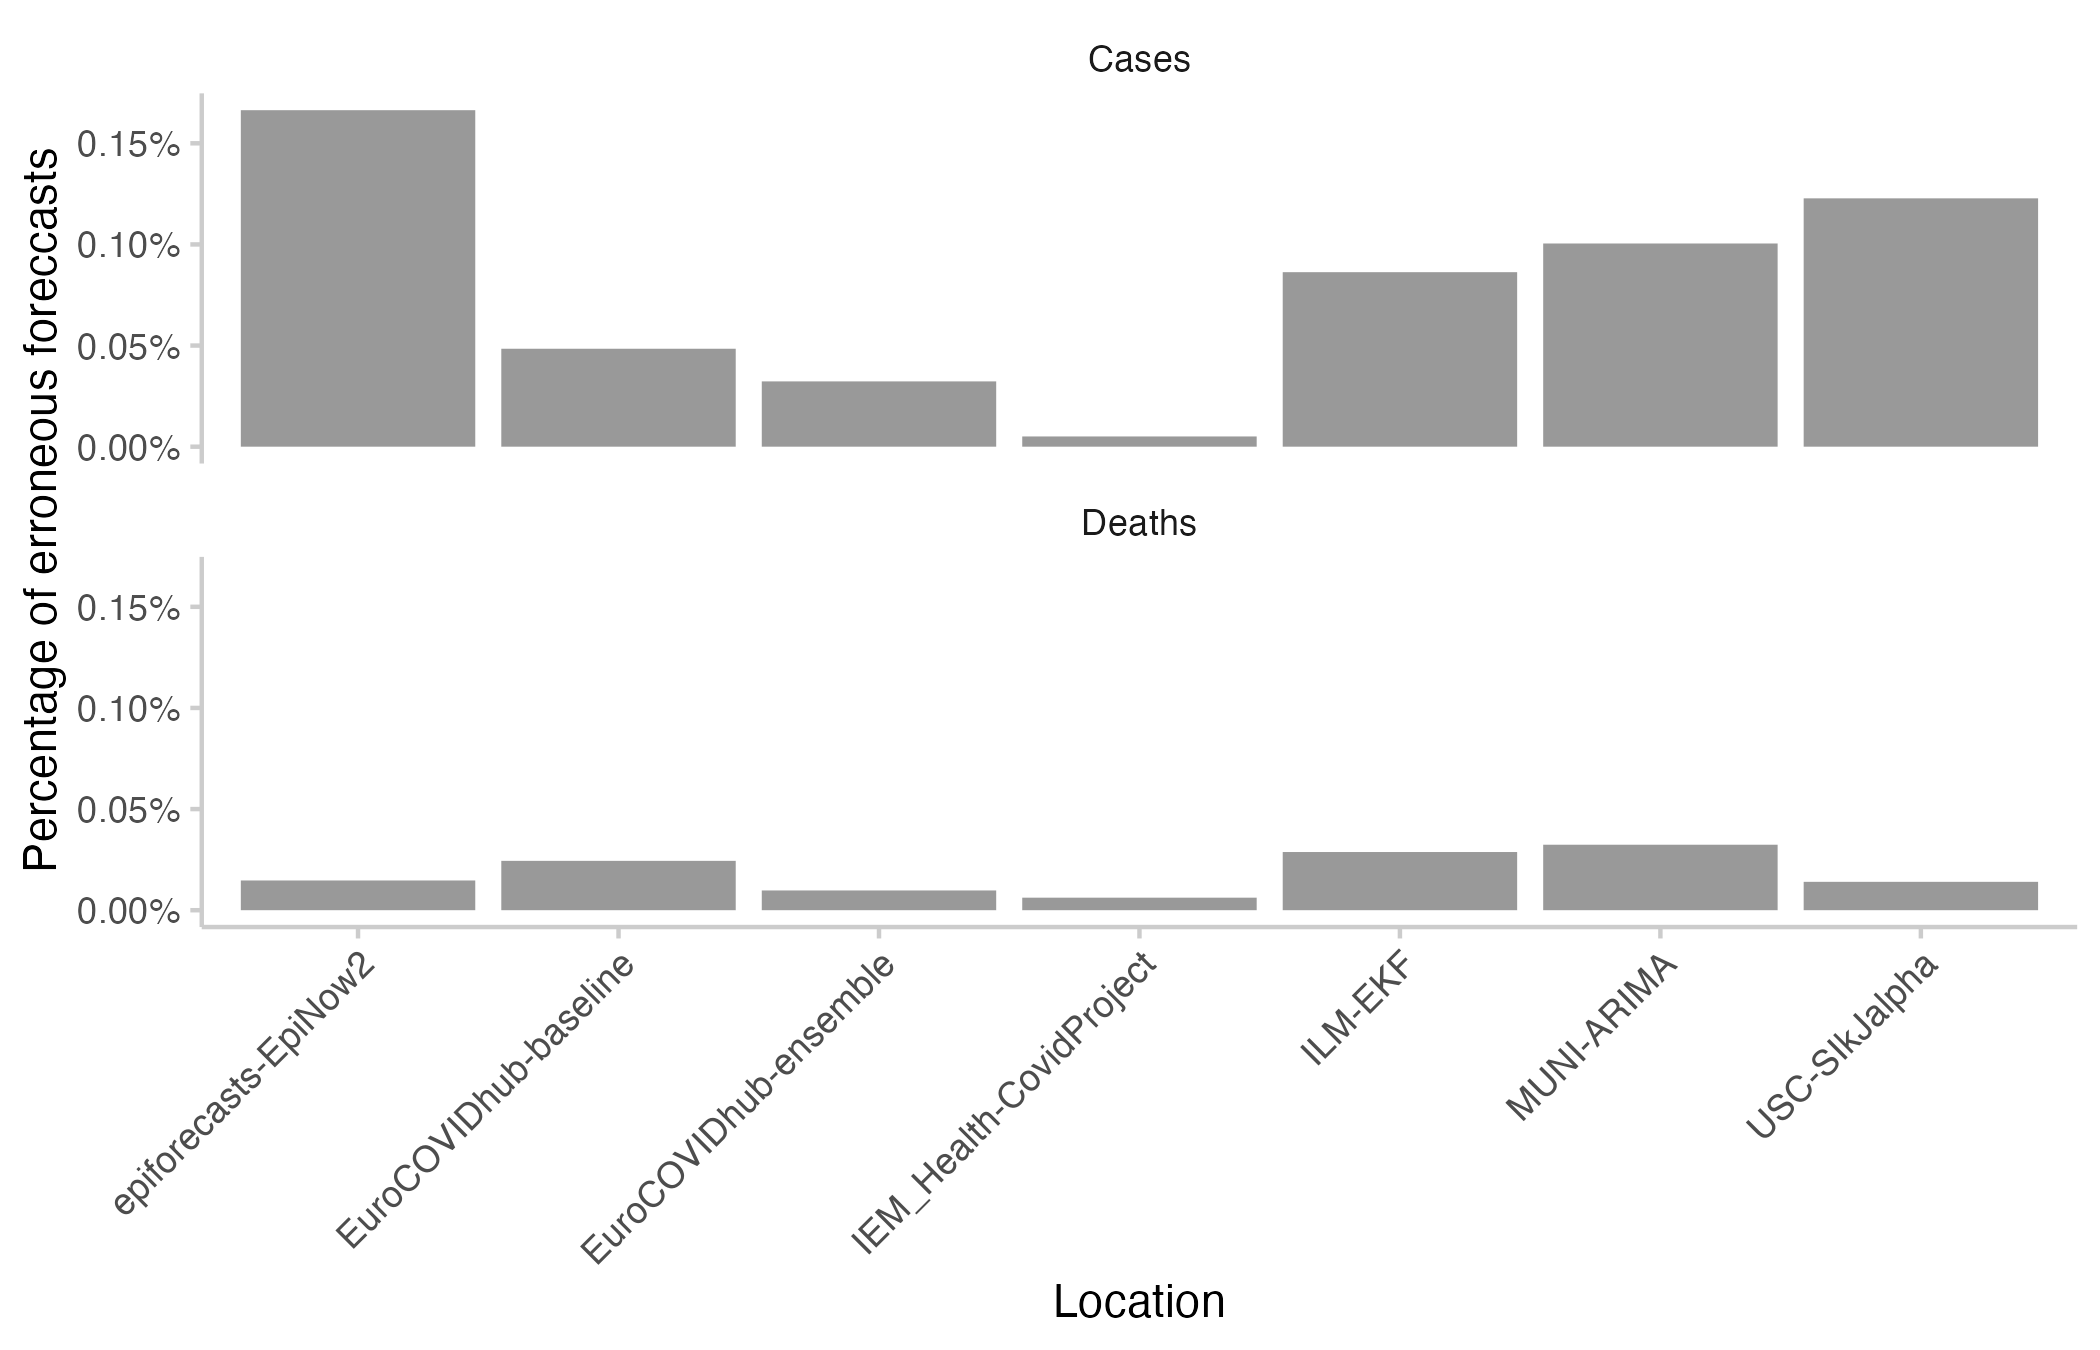
\includegraphics[width=0.99\textwidth]{../output/figures/erroneous-forecasts.png}
    \caption{
    Number of forecasts marked as erroneous and removed. Forecasts that were in extremely poor agreement with the observed values were removed from the analysis according to the criteria shown in Table \ref{tab:erroneous}. 
    }
    \label{fig:erroneous-forecasts}
\end{figure}






\begin{table}
\centering
\begin{tabular}{ccc}
\toprule
True value & \& & Median prediction\\
\midrule
$>0$ & \ & $>100\times$ true value\\
$>10$ & \  & $>20\times$ true value\\
$>50$ & \  & $<1/50\times$ true value\\
$= 0$ & \  & $>100$\\
\bottomrule
\end{tabular}
\caption{Criteria for removing forecasts. Any forecast that met one of the listed criteria (represented by a row in the table), was removed. Those forecasts were removed in order to be better able to illustrate the effects of the log-transformation on scores and eliminating distortions caused by outlier forecasters. When evaluating models against each other (rather than illustrating the effect of a transformation), one would prefer not to condition on the outcome when deciding whether a forecast should be taken into account. }
\label{tab:erroneous}
\end{table}


\begin{figure}[h!]
    \centering
    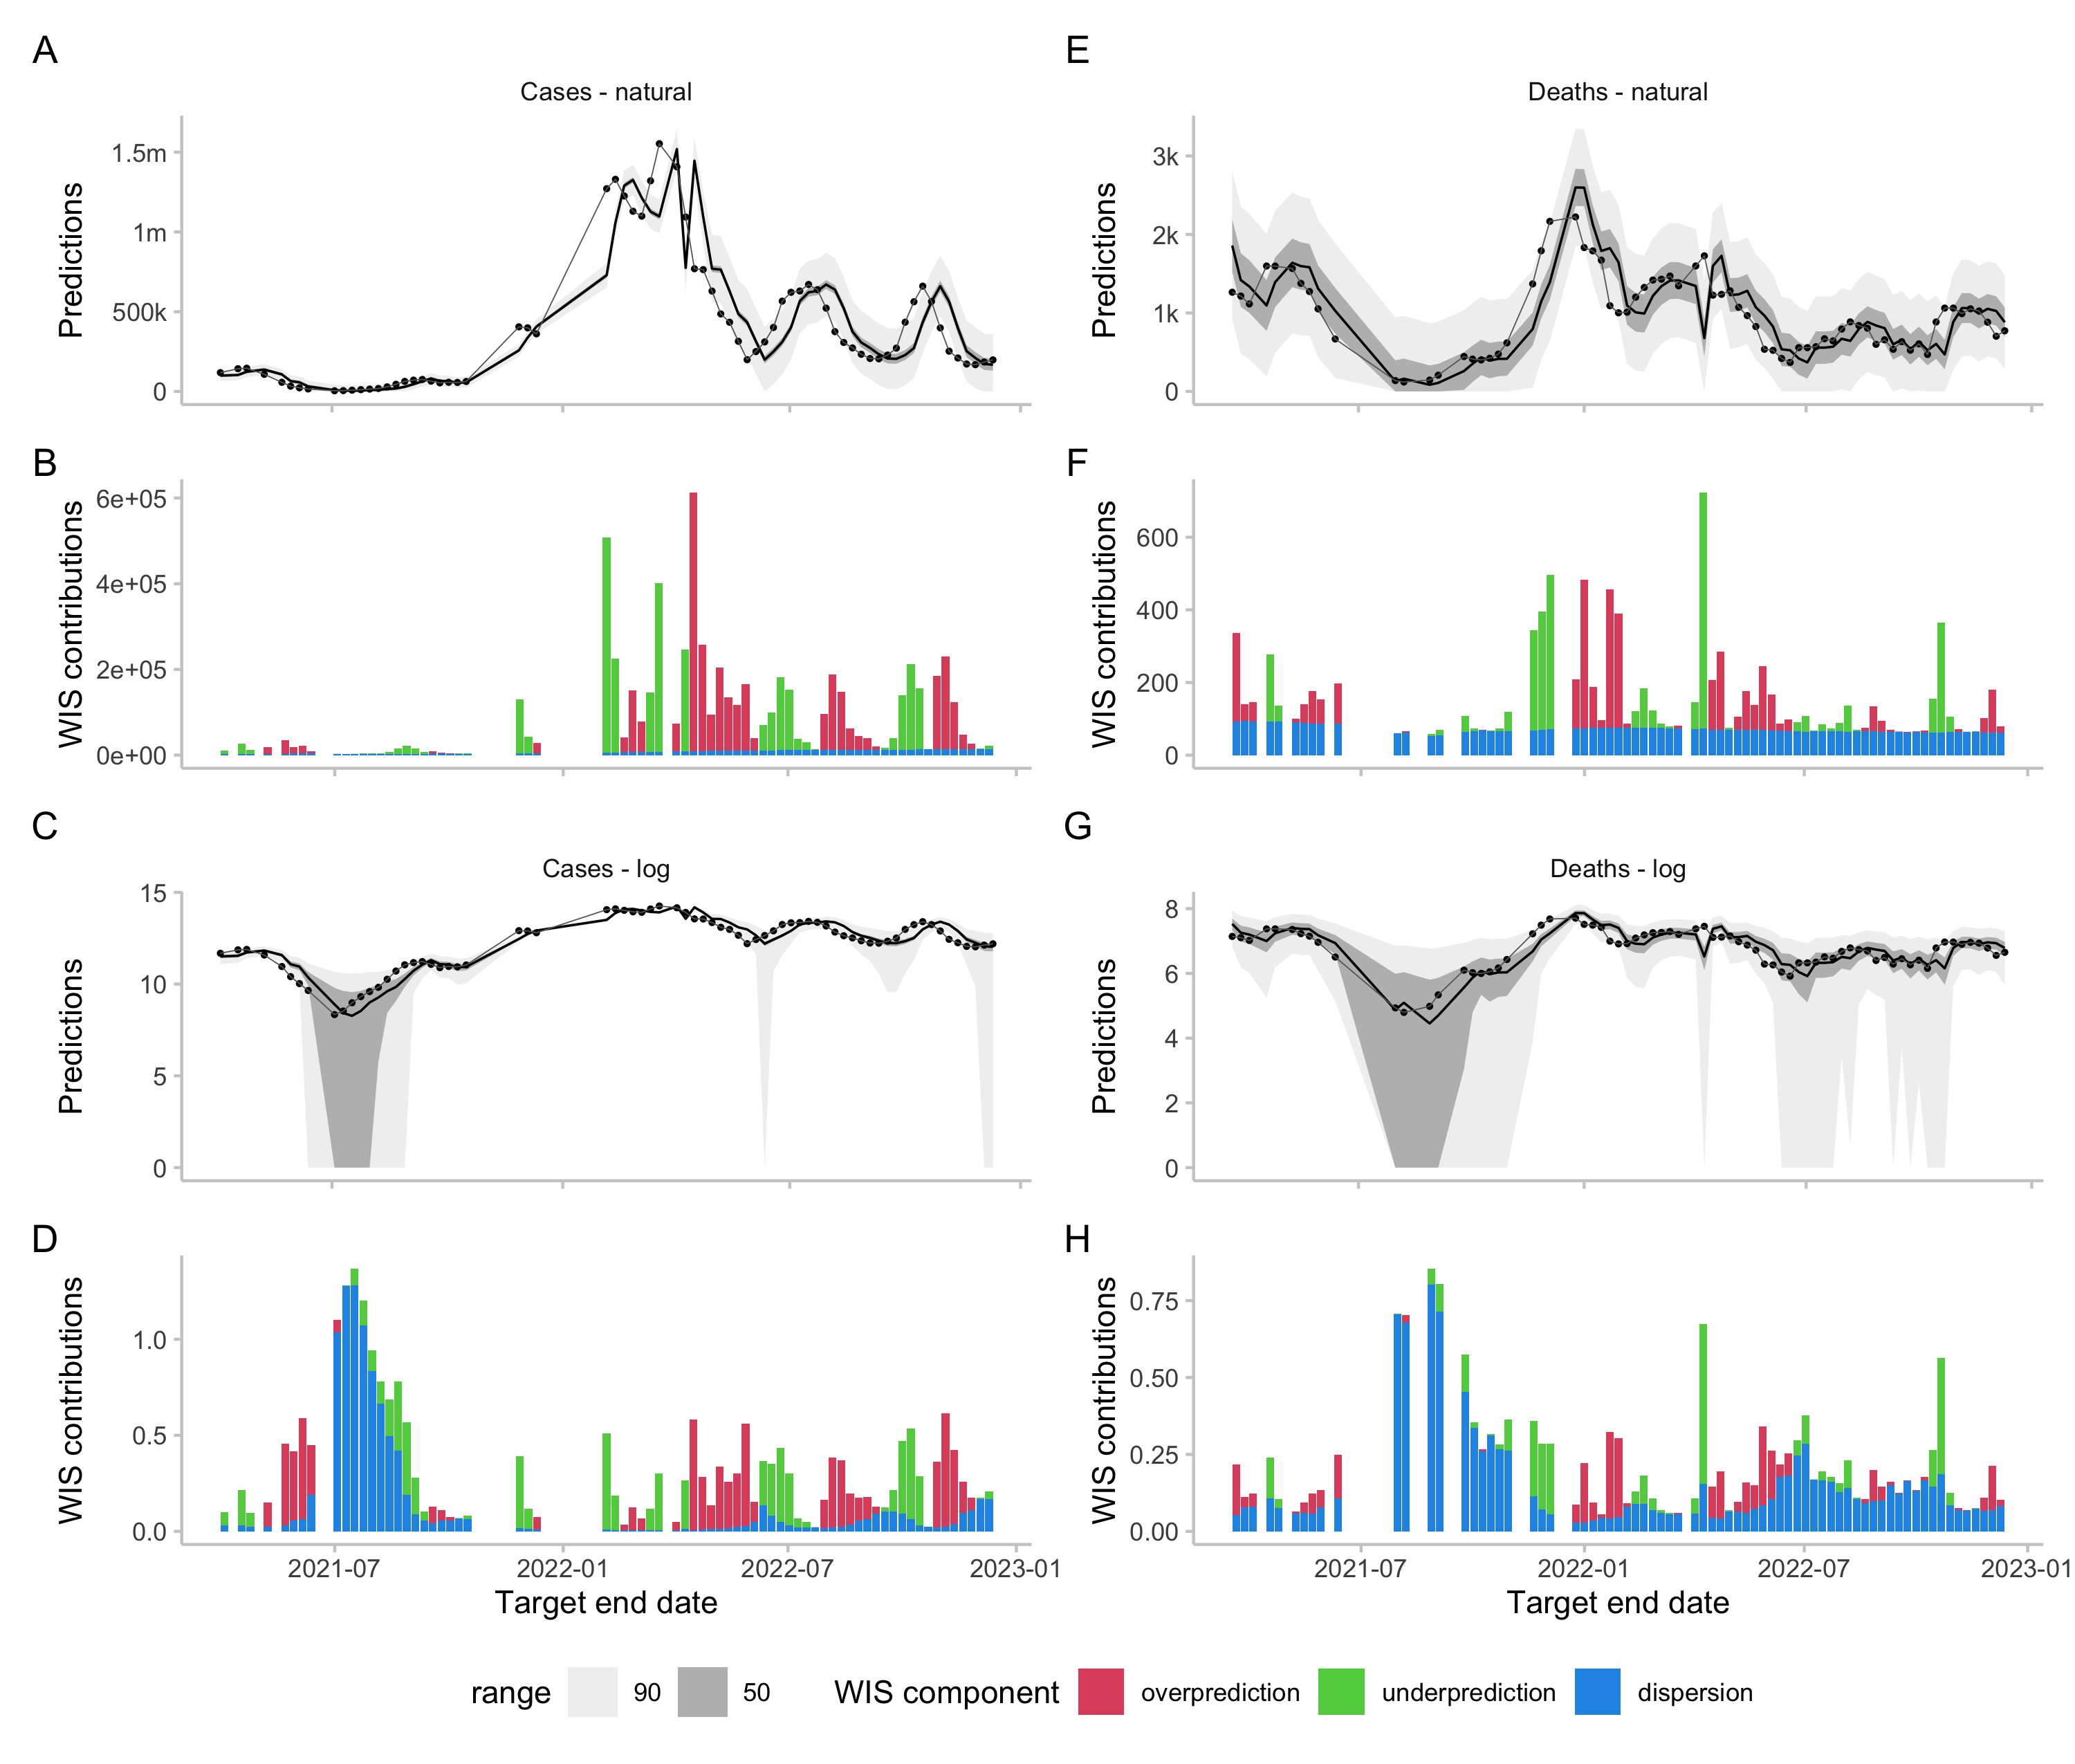
\includegraphics[width=0.99\textwidth]{../output/figures/HUB-model-comparison-baseline.png}
    \caption{
    Forecasts and scores for two-week-ahead predictions from the EuroCOVIDhub-baseline made in Germany. The model had zero included in some of its 50 percent intervals (e.g. for case forecasts in July 2021), leading to excessive dispersion values on the log scale. One could argue that including zero in the prediction intervals constituted an unreasonable forecast that was rightly penalised, but in general care has to be taken with small numbers. One potential way to do deal with this could be to use a higher $a$ value when applying a transformation $\log(x + a)$, for example $a = 10$ instead of $a = 1$. A, E: 50\% and 90\% prediction intervals and observed values for cases and deaths on the natural scale. B, F: Corresponding scores. C, G: Forecasts and observations on the log scale. D, H: Corresponding scores. 
    }
    \label{fig:HUB-model-comparison-baseline}
\end{figure}

\begin{figure}[h!]
    \centering
    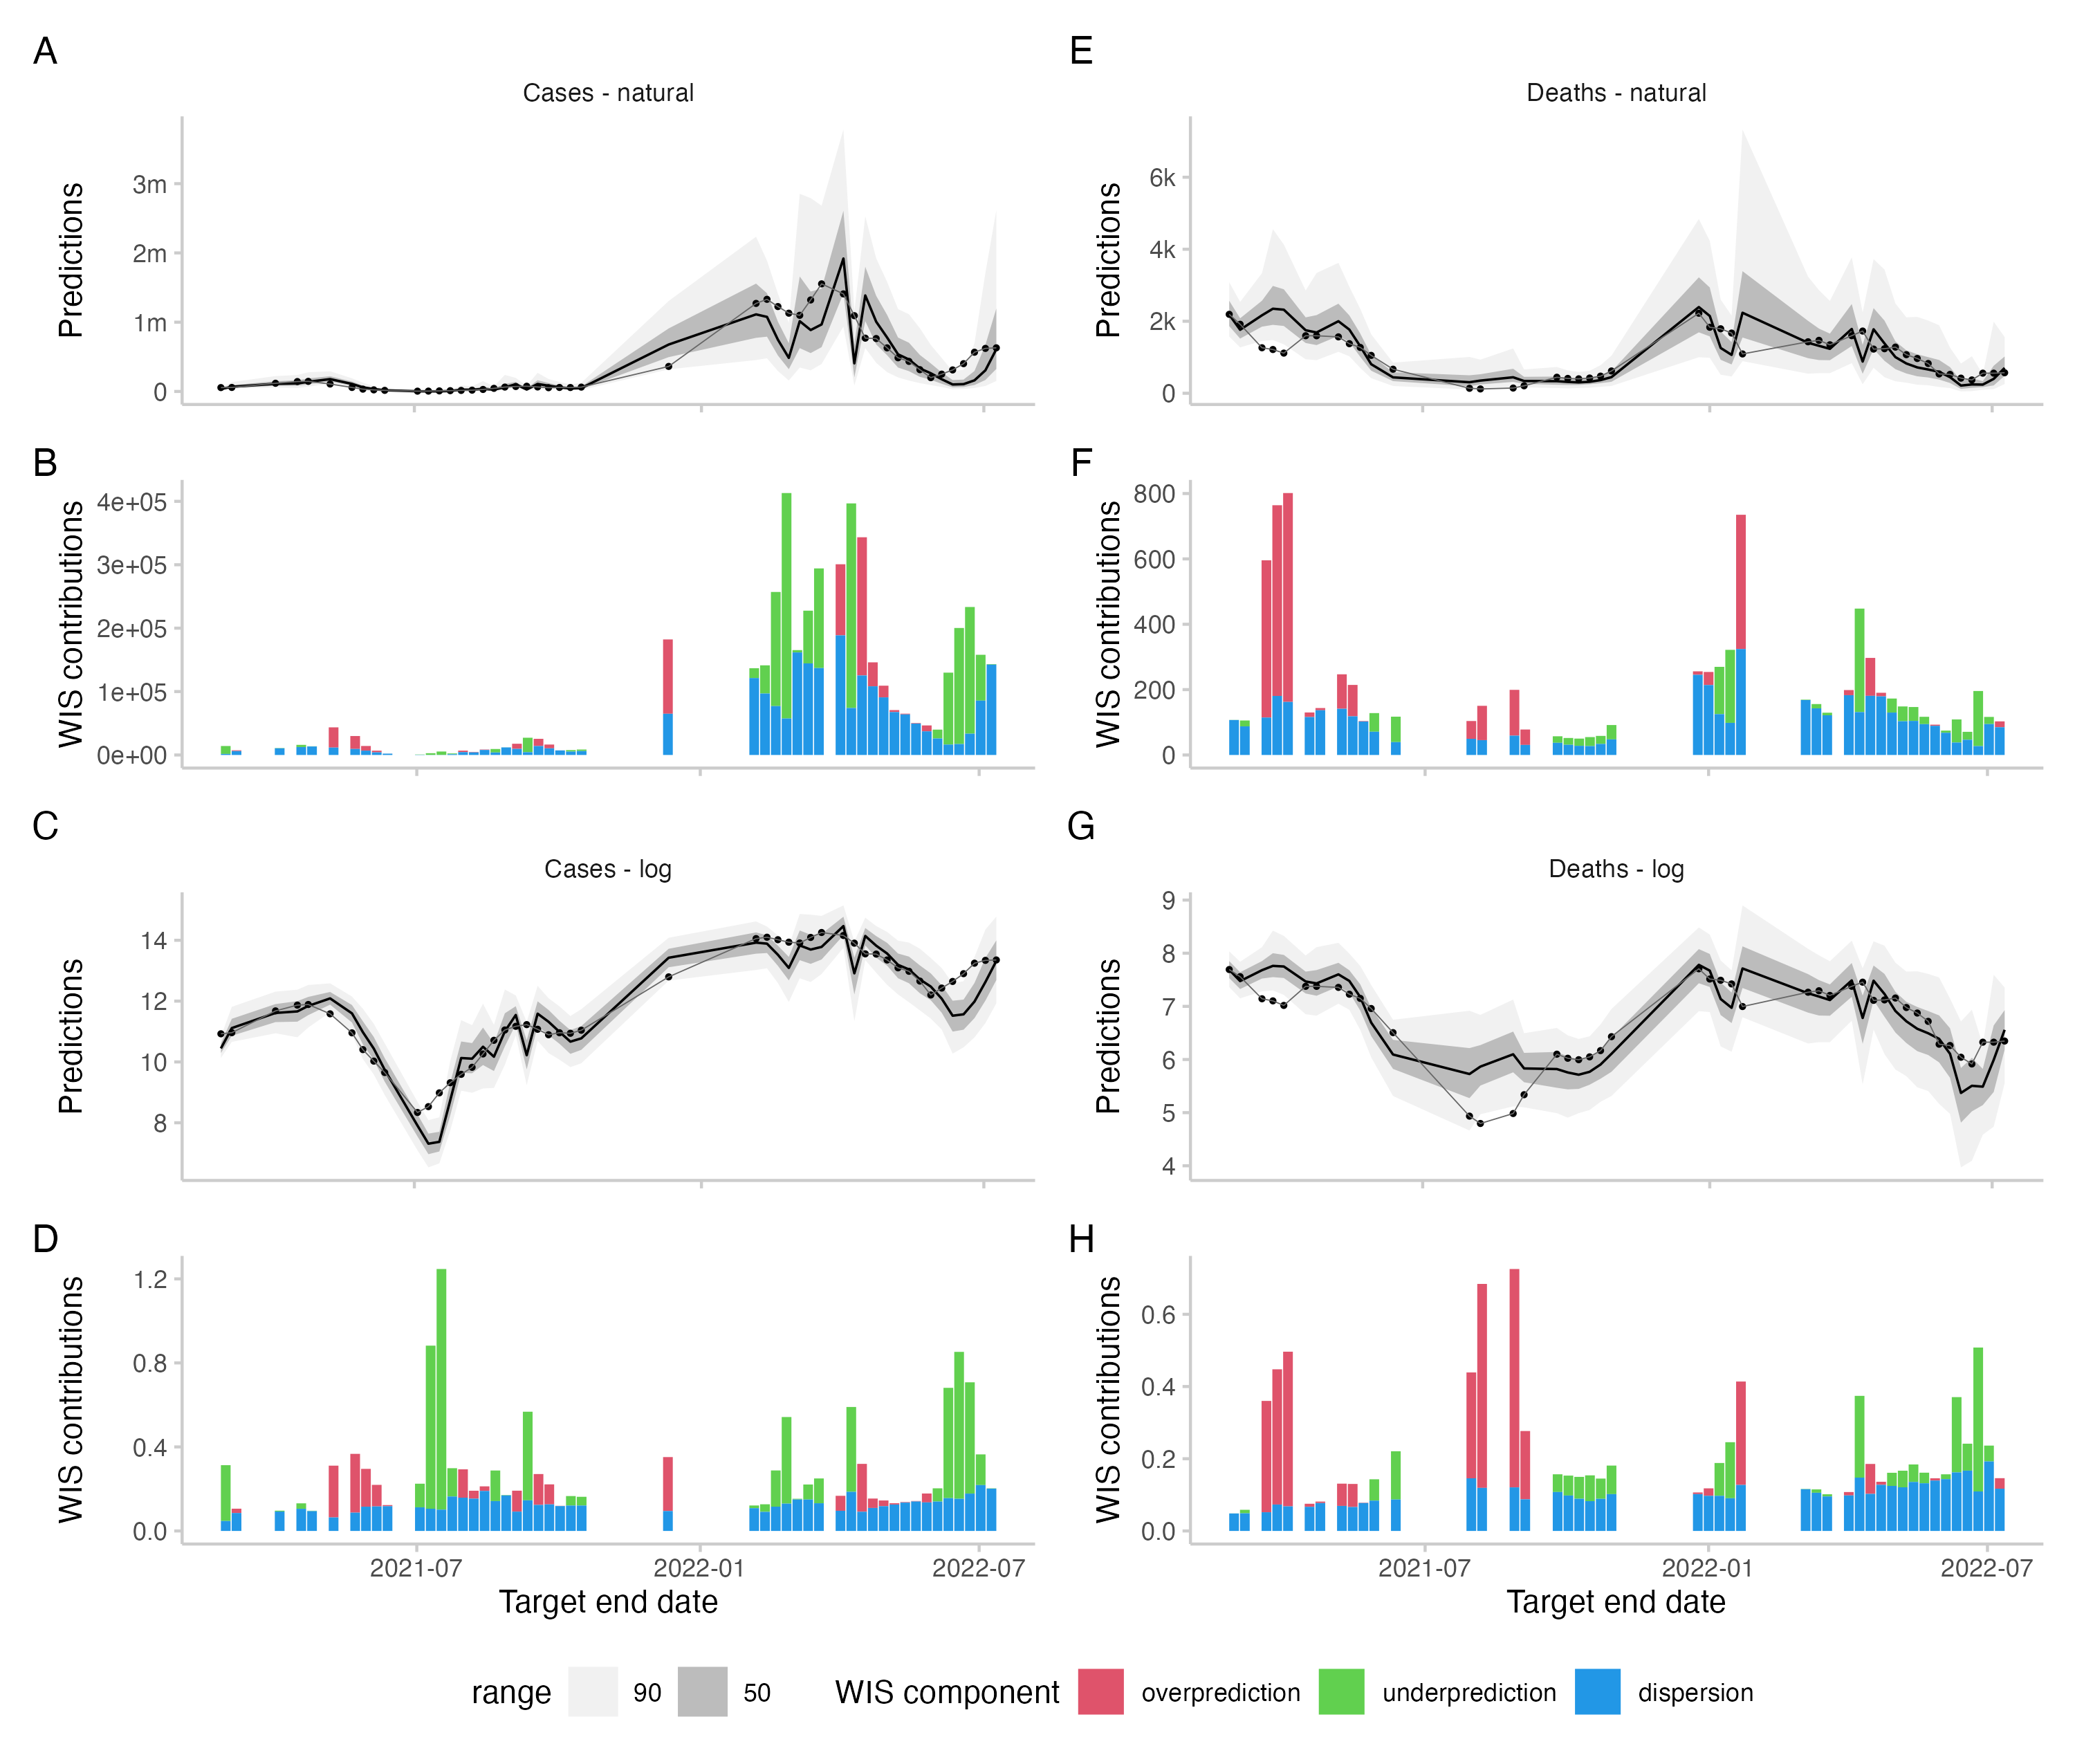
\includegraphics[width=0.99\textwidth]{../output/figures/HUB-model-comparison-epinow.png}
    \caption{
    Forecasts and scores for two-week-ahead predictions from the epiforecasts-EpiNow2 model \citep{epinow2} made in Germany. A, E: 50\% and 90\% prediction intervals and observed values for cases and deaths on the natural scale. B, F: Corresponding scores. C, G: Forecasts and observations on the log scale. D, H: Corresponding scores. 
    }
    \label{fig:HUB-model-comparison-epinow}
\end{figure}




\end{document}